\addchap{Annex}

\begin{appendix}

\begin{minipage}{\linewidth}
\begin{lstlisting}[caption={Example FFmpeg Shell Script}, label=ex:shell, captionpos=b]
#!/usr/bin/env bash

# change directory to this file to  
# make it runnable from anywhere
cd "$(dirname "$0")" || exit
    
# use ENV variables to override configured defaults
OUTPUT="${OUTPUT:-http://localhost:6262/ingest/bbb/source.mpd}"
    
ffmpeg \
    -loglevel error -stats -hide_banner \
    -f lavfi -re -i testsrc=size=1280x720:rate=25 \
    -profile main \
    -pix_fmt yuv420p \
    -map 0:v:0 -s:v:0 1280x720 -b:v:0 2048000 \
-maxrate:v:0 2200000 -bufsize:v:0 3300000 \
    -f dash \
    -dash_segment_type mp4 \
    -preset medium \
    -sc_threshold 0 \
    -r 25 \
    -keyint_min 48 \
    -g 48 \
    -c:v libx264 \
    -hls_playlist 1 \
    -master_m3u8_publish_rate 1 \
    -http_persistent 1 \
    -adaptation_sets "id=0,streams=v" \
    -seg_duration 1.920 \
    -update_period 1.920 \
    -use_template 1 \
    -use_timeline 1 \
    -utc_timing_url https://time.akamai.com/?iso \
    -write_prft 1 \
    -window_size 5 \
    -extra_window_size 0 \
    -flags +global_header \
    -init_seg_name \$RepresentationID\$/segment_init.\$ext\$ \
    -media_seg_name \
\$RepresentationID\$/segment_\$Number%09d\$.\$ext\$ \
    "$OUTPUT"
\end{lstlisting}
\end{minipage}

\begin{figure}
    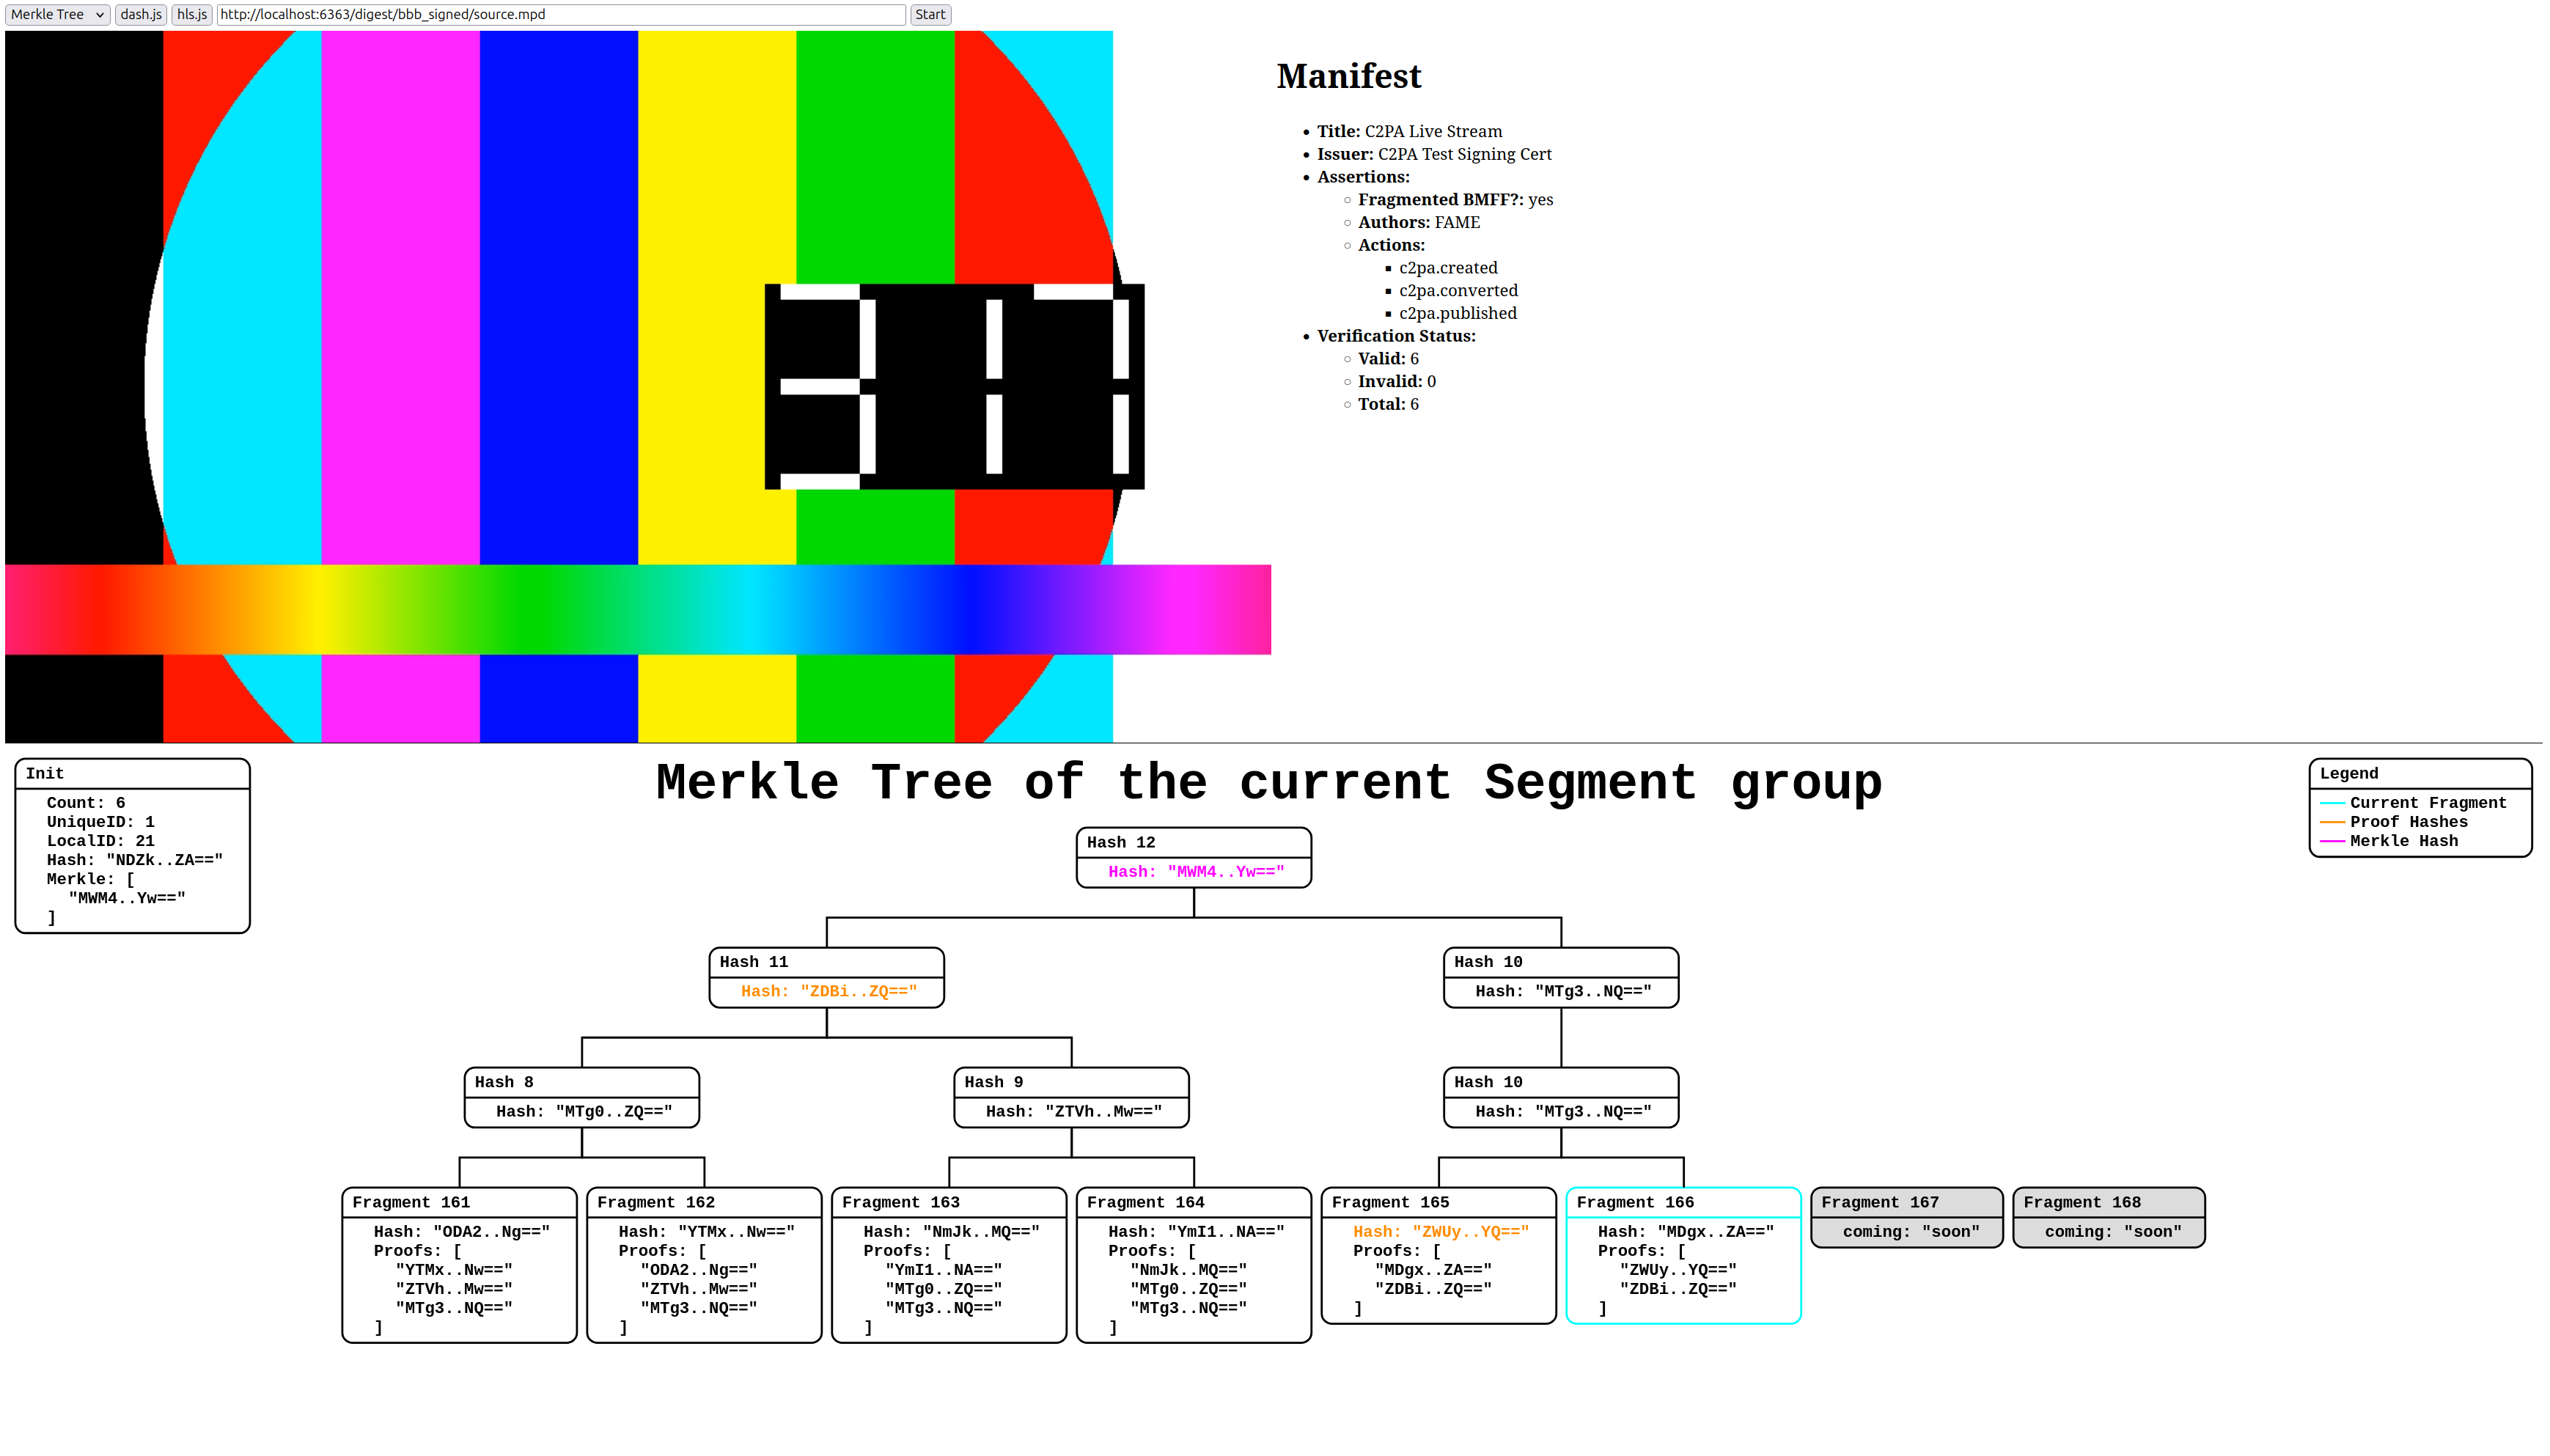
\includegraphics[width=0.95\linewidth, fbox]{merkle-tree-partial.png}
    \caption{Example Rolling Hash Visualization}
    \label{fig:incomple_mt}
\end{figure}

\end{appendix}

\endinput
